\chapter*{Лабораторная работа 7. Утилиты Netcat и Cryptcat}
\addcontentsline{toc}{chapter}{Лабораторная работа 7. Утилиты Netcat и Cryptcat}

\textbf{Цель работы:} Исследовать взаимодействие процессов на разных хостах при помощи утилит Netcat и её защищенного аналога Cryptcat.

\section*{1. Установка}
\addcontentsline{toc}{section}{1. Установка}

Утилита Netcat уже была установлена в рамках предыдущих работ для эмуляции Telnet подключения
\begin{Verbatim}[frame=single]
    smart@thinkpad$ pacman -Qi netcat
    Name            : gnu-netcat
    Version         : 0.7.1-9
    Description     : GNU rewrite of netcat, the network piping application
    Architecture    : x86_64
    URL             : http://netcat.sourceforge.net/
    Licenses        : GPL
    Groups          : None
    Provides        : netcat
    Depends On      : glibc  texinfo
    Optional Deps   : None
    Required By     : None
    Optional For    : None
    Conflicts With  : None
    Replaces        : netcat
    Installed Size  : 66.24 KiB
    Packager        : Felix Yan <felixonmars@archlinux.org>
    Build Date      : Tue 27 Dec 2022 02:47:12 PM MSK
    Install Date    : Wed 08 Feb 2023 11:43:18 PM MSK
    Install Reason  : Explicitly installed
    Install Script  : No
    Validated By    : Signature
\end{Verbatim}

\section*{2. Взаимодействие процессов}
\addcontentsline{toc}{section}{2. Взаимодействие процессов}

Организуем простейшее сетевое взаимодействие двух процессов.

В этом и дальнейших примерах в качества адреса будет использован адрес локального интерфейса, но на практике можно использовать любой маршрутизируемый адрес.

Процесс-сервер будет работать в режиме прослушивания. Для его запуска, будем использовать комманду \texttt{nc -nvlp 1234}, где:

\begin{itemize}
    \item \texttt{-n} -- не выполнять резолвинг имён через DNS
    \item \texttt{-v} -- подробный (verbose) режим отображения логов
    \item \texttt{-l} -- режим прослушивания (в некоторых реализациях netcat, \texttt{-l} завершит сервер после разрыва соединения, \texttt{-L} перезапустит сервер)
    \item \texttt{-p 1234} -- номер порта, на котором ожидается соединение
\end{itemize}

Опционально, можно указать \texttt{-t} для TCP соединения (используется по умолчанию) или \texttt{-u} для UDP.

Запуск сервера и общение с клиентом
\begin{Verbatim}[frame=single]
    smart@thinkpad$ nc -nvlp 1234
    Connection from 127.0.0.1:52880
    Hi from client
    Hi from server
\end{Verbatim}

Для запуска клиента будем использовать комманду \texttt{nc 127.0.0.1 1234}, где:
\begin{itemize}
    \item \texttt{127.0.0.1} -- IP-адрес сервера
    \item \texttt{1234} -- порт, на котором слушает сервер
\end{itemize}

Запуск клиента и общение с сервером
\begin{Verbatim}[frame=single]
    smart@thinkpad$ nc 127.0.0.1 1234
    Hi from client
    Hi from server
\end{Verbatim}

Проверка состояние сокета
\begin{Verbatim}[frame=single]
    smart@thinkpad$ ss -tp | grep nc
    ESTAB 0   0      127.0.0.1:52880          127.0.0.1:search-agent users:(("nc",pid=44033,fd=3))              
    ESTAB 0   0      127.0.0.1:search-agent   127.0.0.1:52880        users:(("nc",pid=43782,fd=4)) 
\end{Verbatim}

Пакеты, пойманные Wireshark
\begin{center}
    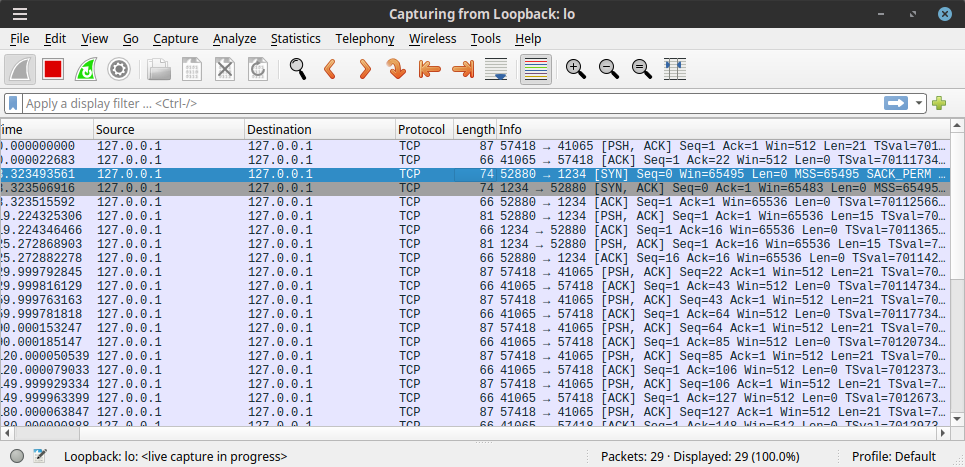
\includegraphics[scale=0.55]{res/7.wireshark-nc-chat.png}
\end{center}

Wireshark позволяет полностью отследить всю переписку
\begin{center}
    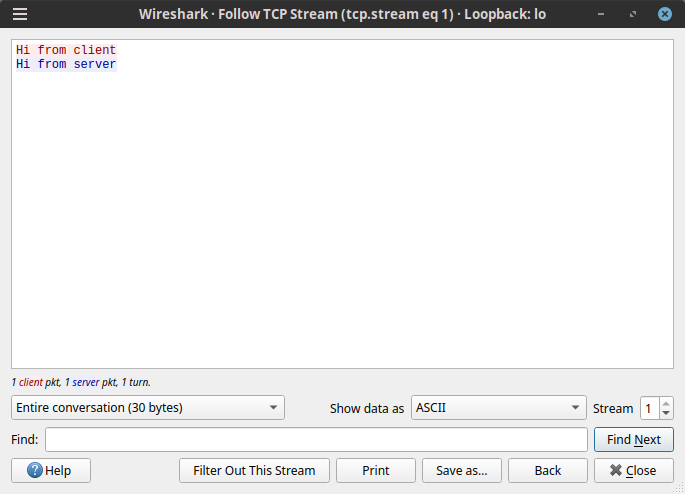
\includegraphics[scale=0.55]{res/7.wireshark-nc-follow.png}
\end{center}

\section*{3. Передача файлов}
\addcontentsline{toc}{section}{3. Передача файлов}

Все следующие примеры (включая сжатие) подразумевают не зашифрованную передачу, это значит Wireshark может перехватить и восстановить передаваемые файлы.

\subsection*{3.1 Передача одного файла}
\addcontentsline{toc}{subsection}{3.1 Передача одного файла}

На принимающей стороне, запускаем прослушивающий сервер \texttt{nc -nvlp 1234 > file.txt}.

Все параметры запуска уже были рассмотрены в предыдущем примере, вывод команды сделан в файл \texttt{file.txt}.

Получение файла
\begin{Verbatim}[frame=single]
    smart@thinkpad$ nc -nvlp 1234 > file.txt
    Connection from 127.0.0.1:56638
\end{Verbatim}

На передающей стороне, делаем такой вызов \texttt{cat file.txt | nc 127.0.0.1 1234}. В некоторых реализациях есть дополнительная опция \texttt{-q 0} для того, что бы netcat автоматически завершил работу сразу после отправки.

Передача файла
\begin{Verbatim}[frame=single]
    smart@thinkpad$ nc 127.0.0.1 1234 < file.txt

\end{Verbatim}

\subsection*{3.2 Передача одного файла с отображением прогресса}
\addcontentsline{toc}{subsection}{3.2 Передача одного файла с отображением прогресса}

Главный минус предыдущего подхода в том, что непонятно когда завершена передача.

Возможным решением может быть добавление счётчика на отправляющий и принимающей стороне.

Получение файла
\begin{Verbatim}[frame=single]
    smart@thinkpad$ nc -nvlp 1234 | pv -b > file.txt
    Connection from 127.0.0.1:36388
     304 B
\end{Verbatim}

Передача файла
\begin{Verbatim}[frame=single]
    smart@thinkpad$ cat file.txt | pv -b | nc 127.0.0.1 1234
    304 B
\end{Verbatim}

При помощи утилиты pv (pipeviewer) мы можем видеть прогресс передачи через подсчёт количества байт (ключ \texttt{-b} просто отображает итоговый объём, отключая анимацию передачи, хотя она бывает полезна при передаче больших объёмов).

\subsection*{3.3 Передача нескольких файлов}
\addcontentsline{toc}{subsection}{3.3 Передача нескольких файлов}

Для передачи нескольких файлов в одной директории можно написать простой bash-скрипт, который переберёт все файлы, и для каждого сделает вызод nc.

Другой вариант передачи -- запаковать её в тарбол на одном конце, и распаковать на другом. Кроме прочего, это позволит передать и права, выставленные на файлы.

Получение директории
\begin{Verbatim}[frame=single]
    smart@thinkpad$ nc -nvlp 1234 | pv -b | tar xf -
    Connection from 127.0.0.1:35942
    39.0MiB
\end{Verbatim}

Тут мы используем утилиту tar:

\begin{itemize}
    \item \texttt{x} -- производить операцию извлечения из обрабатываемого потока
    \item \texttt{f} -- обрабатывать архивный файл
    \item \texttt{-} -- вместо имени архива поток, полученный из пайпа
\end{itemize}

Передача директории
\begin{Verbatim}[frame=single]
    smart@thinkpad$ tar cf - . | pv -b | nc 127.0.0.1 1234
    39.0MiB
\end{Verbatim}

Тут мы используем утилиту tar:

\begin{itemize}
    \item \texttt{с} -- производить операцию сжатия
    \item \texttt{f} -- обрабатывать архивный файл
    \item \texttt{-} -- вместо файла, передаём данные в пайп
    \item \texttt{.} -- обрабатываем все файлы в текущей директории
\end{itemize}

\subsection*{3.4 Передача нескольких файлов со сжатием}
\addcontentsline{toc}{subsection}{3.4 Передача нескольких файлов со сжатием}

Для экономии трафика, можно сражу сжимать поток любым архиватором. Тема выбора подходящего архиватора для различных типов данных достойна отдельного исследования, мы будем использовать gzip, как оптимальное решение между скоростью работы, качеством сжатия и количеством потребляемых ресурсов. Для этого достаточно передать параметр \texttt{z} утилите tar.

Получение директории со сжатием
\begin{Verbatim}[frame=single]
    smart@thinkpad$ nc -nvlp 1234 | pv -b | tar xzf -
    Connection from 127.0.0.1:43324
    36.8MiB
\end{Verbatim}

Передача директории
\begin{Verbatim}[frame=single]
    smart@thinkpad$ tar czf - . | pv -b | nc 127.0.0.1 1234
    36.8MiB
\end{Verbatim}

Удалось уменьшить объём передаваемого трафика с 39.0MiB до 36.8MiB (экономия больше 5\%!).

\subsection*{3.5 Передача образа жёского диска}
\addcontentsline{toc}{subsection}{3.5 Передача образа жёского диска}

Иногда необходимо сделать резервную копию образа жёсткого диска с одной машины на другую.

В таком случае, для отправки образа можно использовать такую команду \texttt{bzip2 -c /dev/sdb1 | nc -nvlp 1234}. Эта команда будет пересылать все данные с диска \texttt{/dev/sdb1}. Учитывая, что мы читаем диск как набор секторов (в двоичном формате), для сжатия будем использовать \texttt{bzip2}.

Со стороны получателя, будет распаковывать поток и складывать в отдельный файл \texttt{nc 192.168.1.102 1234 | pv -b | bzip2 -d > hdImage.img}

\section*{4. Защищенное взаимодействие}
\addcontentsline{toc}{section}{4. Защищенное взаимодействие}

\subsection*{4.1 Установка cryptcat}
\addcontentsline{toc}{subsection}{4.1 Установка cryptcat}

Утилита cryptcat довольно специфичная. Её нет в стандартном репозитории для моего дистрибутива linux (Arch linux) и нет а пользовательских пакетах (AUR). Дистрибутив Kali linux использует довольно старую версию пакета (\texttt{20031202}), но на официальном сайте (\url{https://cryptcat.sourceforge.net/}) есть ссылка на sourceforge, где размещена версия от октября 2005-го года.

Берём исходники утилиты по ссылке
\url{https://sourceforge.net/projects/cryptcat/files/cryptcat-unix-1.2/cryptcat-unix-1.2.1/cryptcat-unix-1.2.1.tar/download}

Изучение исходников показывает, что по сути это старая версия утилиты Netcat для которой имплантирован модуль twofish2. Примечания к релизу содержат некоторое количество известных багов, которые планируется решить когда-то в будущем.

Сборка из исходников сыпет большим количеством предупреждений, т.к. код был написан на более старую версию API glibc.

\subsection*{4.2 Взаимодействие процессов}
\addcontentsline{toc}{subsection}{4.2 Взаимодействие процессов}

Повторим эксперимент с созданием чата.

Запуск сервера и общение с клиентом
\begin{Verbatim}[frame=single]
    smart@thinkpad$ ./cryptcat -nvlp 1234
    listening on [any] 1234 ...
    connect to [127.0.0.1] from (UNKNOWN) [127.0.0.1] 39944
    hello from client
    hello from server
\end{Verbatim}

Запуск клиента и общение с сервером
\begin{Verbatim}[frame=single]
    smart@thinkpad$ ./cryptcat 127.0.0.1 1234
    hello from client
    hello from server
\end{Verbatim}

Проверка состояние сокета
\begin{Verbatim}[frame=single]
    smart@thinkpad$ ss -tp | grep nc
    ESTAB 0   0      127.0.0.1:39944          127.0.0.1:search-agent users:(("cryptcat",pid=71954,fd=3))
    ESTAB 0   0      127.0.0.1:search-agent   127.0.0.1:39944        users:(("cryptcat",pid=71953,fd=4))
\end{Verbatim}

Пакеты, пойманные Wireshark
\begin{center}
    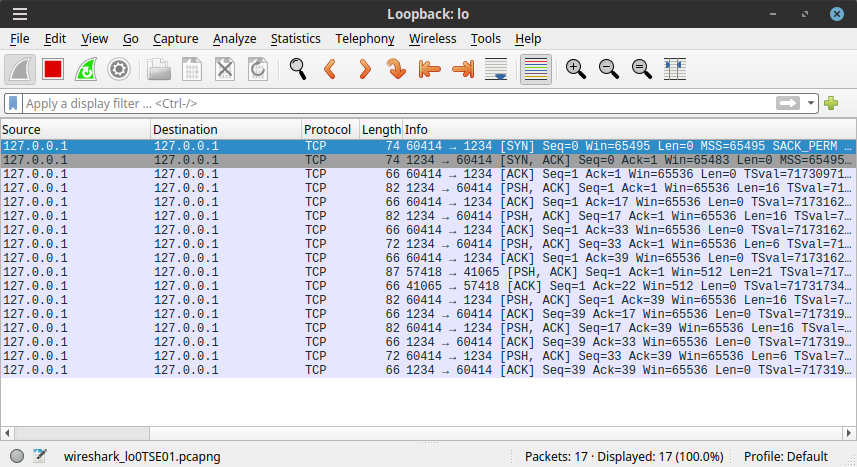
\includegraphics[scale=0.55]{res/7.wireshark-cryptcat-chat.png}
\end{center}

Wireshark показывает, что данные переданы в зашифрованном виде
\begin{center}
    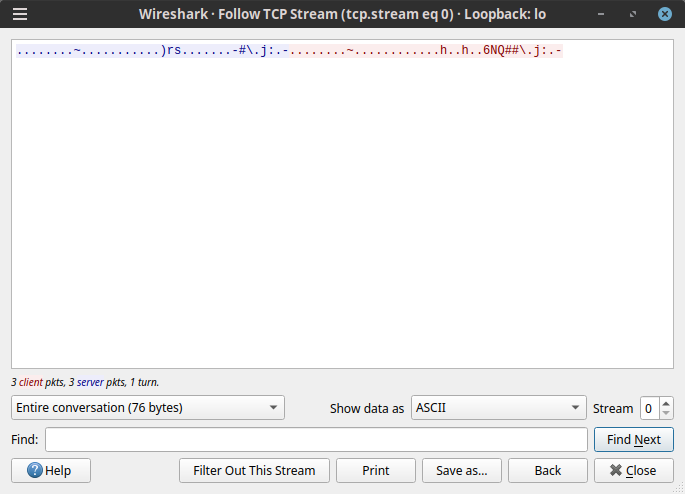
\includegraphics[scale=0.55]{res/7.wireshark-cryptcat-follow.png}
\end{center}

\subsection*{4.3 Передача файлов}
\addcontentsline{toc}{subsection}{4.3 Передача файлов}

Передача файлов работает аналогично Netcat, данные зашифрованы.

Получение файла
\begin{Verbatim}[frame=single]
    smart@thinkpad$ ../cryptcat -nvlp 1234 | pv -b > file.txt
    listening on [any] 1234 ...
    connect to [127.0.0.1] from (UNKNOWN) [127.0.0.1] 54856
    304 B
\end{Verbatim}

Передача файла
\begin{Verbatim}[frame=single]
    smart@thinkpad$ cat file.txt | pv -b | ./cryptcat 127.0.0.1 1234
    304 B
\end{Verbatim}

\section*{5. Direct Network Traffic}
\addcontentsline{toc}{section}{5. Direct Network Traffic}

Выполним установку двунаправленного пайпа для редиректа локального порта 1234 на 80-й порт google.

Для начала определим, что должно получиться в итоге. При запросе на 80-й порт, google отвечает 301 и отправляет устанавливать https соединение. Но даже такого ответа нам достаточно для теста.

\begin{Verbatim}[frame=single]
    smart@thinkpad$ curl google.com
    <HTML><HEAD><meta http-equiv="content-type" content="text/html;charset=utf-8">
    <TITLE>301 Moved</TITLE></HEAD><BODY>
    <H1>301 Moved</H1>
    The document has moved
    <A HREF="http://www.google.com/">here</A>.
    </BODY></HTML>
\end{Verbatim}

Подготовм двунаправленный пайп.
\texttt{nc -l -p 1233 | nc www.google.com 80 | nc -l -p 1234}

После этого, через curl вначале сделаем запрос на порт 1233, потом прочитаем ответ с порта 1234.

Результат работы пайпа
\begin{Verbatim}[frame=single]
    smart@thinkpad$ nc -lp 1233 | nc google.com 80 | nc -lp 1234
    GET / HTTP/1.1
    Host: 127.0.0.1:1234
    User-Agent: curl/7.87.0
    Accept: */*
\end{Verbatim}

Результат работы curl
\begin{Verbatim}[frame=single]
    smart@thinkpad$ curl 127.0.0.1:1233
    ^[[A^C
    smart@thinkpad$ curl 127.0.0.1:1234
    <HTML><HEAD><meta http-equiv="content-type" content="text/html;charset=utf-8">
    <TITLE>301 Moved</TITLE></HEAD><BODY>
    <H1>301 Moved</H1>
    The document has moved
    <A HREF="http://www.google.com:1233/">here</A>.
    </BODY></HTML>
\end{Verbatim}

Естественно, весь трафик ходит незащищенным.

\section*{Выводы}
\addcontentsline{toc}{section}{Выводы}

В этой работе мы познакомились с возможностями утилиты netcat и её безопасной (но, не поддерживаемой) версии cryptcat.

С практической точки зрения, для передачи файлов удобнее использовать rsync (он безопасный и имеет множество полезных опеций), безопасно туннелировать трафик можно при помощи ssh, а локальный редирект портов можно осуществлять средствами встроенного фаервола.